\chapter{Graphs}
\label{chp:graphs}
In this chapter are introduced the fundamentals concepts of \textbf{graphs} as mathematical objects, and as an abstract data type, its applications in computer science, and the most important and notable algorithms with their implementation. 
 
\section{General Definitions}
A graph is a discrete mathematical structure in which the connections between its elements, and their relationship are highlighted. A graph is made up by two different elements: \textbf{nodes} or \textbf{vertices}, and \textbf{links} or \textbf{edges}. In case the links do not have any direction the graph is called \textbf{undirected graph} (Figure), in case instead the links have a direction the graph is called \textbf{directed graph}.

\begin{figure}[H]
	\begin{center}
		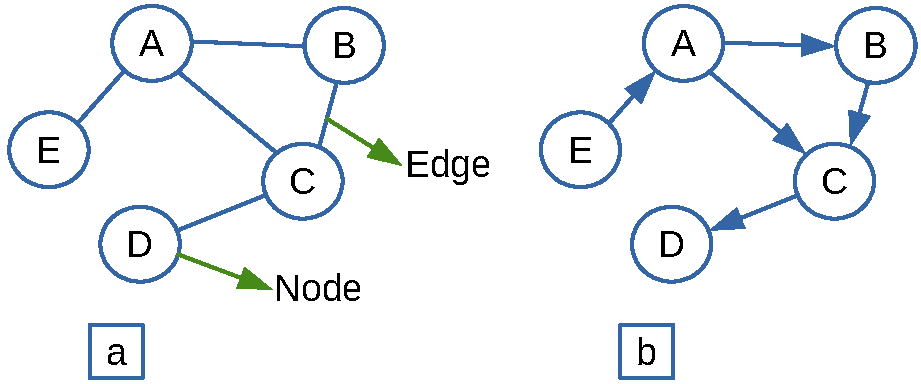
\includegraphics[scale=.6]{chapters/graphs/images/graphs_1.pdf}
		\caption[Undirected (a) and directed (b) graphs and its elements.]{Undirected (a) and directed (b) graphs and its elements.}
		\label{graphs_1}
	\end{center}
\end{figure}

Formally a graph is the pair \(G=(V, E)\), where \(V\) is the set of all vertices, and \(E\) is the set of paired vertices, whose elements are called edges \cite{wikigraphmath} (\href{https://en.wikipedia.org/wiki/Graph_(discrete_mathematics)}{Graph, Wikipedia}).

A \textbf{tree} (Chapter \ref{chp:trees}) is a special kind of graph.

Graphs are very useful to describe a lot of real situations like: connections between people, computers (internet), web pages (world wide web), airports, cities, and gene inside the DNA.

In graphs, differently to trees, closed loops can exist. These kind of closed loops can be dangerous for the algorithms because they could lead to infinite executions.

\subsection{Connectivity}
\textbf{Connectivity} is a measure that describe how much the nodes of a graph are connected. It is defined as the minimum number of elements (nodes or edges) that need to be removed to separate the remaining nodes into isolated subgraphs \cite{wikiconnectivity} (\href{https://en.wikipedia.org/wiki/Connectivity_(graph_theory)}{Connectivity, Wikipedia}).

A graph is said to be \textbf{connected} if every pairs of nodes are connected. Thus it always exists at least one path that connects every pairs of nodes. If an undirected graphs is not connected then it is \textbf{disconnected}: in this case there is one or more nodes that can not be reached by any paths.

\paragraph{Strongly Connected}
A directed graph is said to be \textbf{strongly connected} if every pairs of nodes can be reached by one or more path.

\paragraph{Weakly Connected}
A directed graph is said to be \textbf{weakly connected} if by replacing all the direct edges with undirectd ones, the new graph is connected. in a directed graph some nodes can not be reached if all the edges exit or enter from them. The graph in Figure \ref{graphs_2} is weakly connected because the node \(U\) has only entering edges.

\begin{figure}[H]
	\begin{center}
		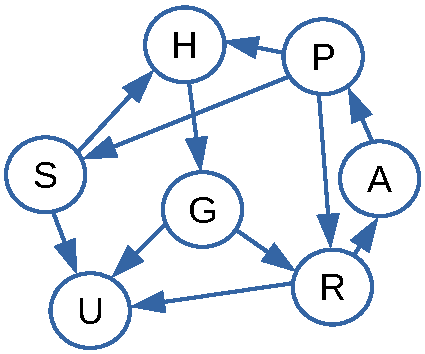
\includegraphics[scale=.6]{chapters/graphs/images/graphs_2.pdf}
		\caption[A weakly connected graph.]{A weakly connected graph.}
		\label{graphs_2}
	\end{center}
\end{figure}

\subsection{Graph Representations}
\cite{wikigraphabstracttype} (\href{https://en.wikipedia.org/wiki/Graph_(abstract_data_type)}{Graph (abstract data type), Wikipedia})